\documentclass[a4paper,10pt]{article}
\usepackage[english]{babel}
\usepackage[utf8]{inputenc}
\usepackage[toc,page]{appendix}
\usepackage{graphicx}

%Includes "References" in the table of contents
\usepackage[nottoc]{tocbibind}
\usepackage{titling}
\usepackage{setspace}

\parskip .8ex

\setlength{\droptitle}{-15em}

%Begining of the document
\begin{document}

\title{\textbf{CSCM35: Big Data and Data Mining \\Coursework 1}}
\date{09/04/20}
\author{Andy Gray\\445348}

\maketitle

\section{Introduction}

We have a practical task assigned to us, that is related to the field of data mining. This task aims to use the association rule, a rule-based machine learning technique, to discover interesting relationships within the provided large dataset. We will be creating to code process the data, as well as analysing the results to see if any insights can be gains and possible reasons to why these might be the case. Throughout this paper we will be explaining our understanding of the problems related to mining data for common patterns while performing visualisations and statistical analysis, as well as applying the association rule mining algorithm on the data, to be able to analyse the outcomes.

Data mining is a necessary part of obtaining knowledge through discovery in databases (KDD). KDD is the term used for the overall process, that involves turning the raw data into useful information. Data mining tasks split into two main categories. These are predictive and descriptive tasks. However, these two main categories split further into four core mining task. These four tasks are cluster analysis, predictive modelling, anomaly detection and association analysis \cite{tan2016introduction}. We will be focusing on the association analysis within this paper.

[Needs expanding about overview of results]

We will first look at the algorithms used within the methodology, explaining how they work and what is the maths formulas behind them driving the algorithm. We will then explain the dataset, and the data preprocessing that occurred, followed by an explanation of the packages used and the parameters set for the algorithms. We will then explain the results and then discuss them and what insights we might have gained. To end, we will be then concluding what we have found.

\section{Proposed Solution}

\subsection{Algorithms Used Explanation}

The first algorithm that we used is one that is from the frequent itemset mining methods, called Apriori \cite{han2011data}. Apriori is an unsupervised learning machine learning algorithm proposed by R. Agrawal and R. Srikant in 1994 \cite{agrawal1994fast, geron2019hands}. The algorithm focuses on using boolean association rules \cite{agrawal1994fast} from using prior knowledge of itemsets that contain the frequent properties. Apriori uses a level-wise search, which operates an iterative approach, where $k$-itemsets get used for exploring $(k+1)$-itemsets \cite{jingjingslides}. In order to improve efficiency, which will reduce the search space, an important characteristic called the Apriori property needs to be applied \cite{han2011data}. 

The Apriori property has a two-step process which involves the join and prunes step. For this explanation, $F_k$ represents the $k$-itemset where $L_k$ represents the candidate for the $k$-itemset. The process of joining is to generate a new itemset, $L_{k+1}$, from the $F_K$ itemset. While the pruning stage aims to identify the itemsets in $L_{k+1}$ that are infrequent from $k$, and then remove them \cite{jingjingslides}. What indicates if the item is infrequent depends on the support count, which is predefined beforehand. Therefore what the algorithm does, is: Let us assume that $k=1$ and a support count of 2, we generate a frequent itemset, at first 1, which we will refer to as $F_1$. What this is doing is scanning the dataset to figure out the count of each occurrence of each item. The next step is the merge, or join, the datasets. Using $F_k$ we can then create $L_{k+1}$. We then prune the data based on the support count eliminating any data that is infrequent, therefore leaving any data that is classed as frequent, adding it to $F_{k+1}$. This process is repeated until $F_k$ is empty \cite{jingjingslides, han2011data}.

The second algorithm that we have used is called the association rule. Rakesh Agrawal, Tomasz Imieli{\'n}ski and Arun Swami developed the algorithm in 1993 \cite{agrawal1993mining}. The association rule algorithm is an unsupervised machine learning algorithm \cite{geron2019hands}. What this algorithm focuses around is the support of the datasets' items and the confidence of the association. The math formula for the support is $support(A \Rightarrow B) = P(A \cup B)$, and the math formula for the confidence is $confidence(A \Rightarrow B) = P(B|A)$.  Similar to the apriori, the support count will drop any relationships that do not meet the desired count. The formula to figure out if the relationships meet the support count is $confidence(A \Rightarrow B) = P(B|A) = \frac{support(A \cup B)}{support(A)} = \frac{support\_count(A \cup B)}{support\_count(A)}$ \cite{jingjingslides, han2011data}. However, the association rule relies on a procedure, like the apriori algorithm, to have been implemented on the dataset first before it can work effectively. While the association rule requires the support threshold, the confidence level, which we can use to make decisions based on the links, can be changed to additional metrics. The metric can be several different ones like conviction and leverage, the one that we will focus on is lift. The metric lift was introduced in 1997 by Sergey Brin, Rajeev Motwani, Jefferey D. Ullman and Shalom Tsur \cite{brin1997dynamic}. This metric figures out how the antecedent and consequent of a rule, $A \rightarrow C$, would occur together and not as statistically independent items. The lift score would indicate if A and C are independent by having a score of exactly 1. The math formula for lift is constructed as $lift(A \rightarrow C) = \frac{confidence(A \rightarrow C)}{support(C)}, range[0, \infty]$ \cite{brin1997dynamic, jingjingslides}.

Overall the apriori algorithm will reduce the dataset by pruning it. The amount of pruning depends on the support count threshold that is applied. This will create the required frequent itemset which the association rule requires. The association rule will then go through the frequent itemset to acquire any patterns of items based on the support count and the metric. In our case, this is the lift or confidence metric.

\subsection{Dataset and Data Preprocessing}

The dataset that has we have acquired is a shopping dataset. It is 44MB in size and is in the format of CSV. There are eight attributes, within the dataset, with 541,910 records. The attributes are InvoiceNo, StockCode, Description, Quantity, InvoiceDate, UnitPrice, CustomerId, Country. There are 4,335 unique customers, 1,8405 individual invoices, 3,659 unique stock items and 37 unique countries.

The purpose of data preprocessing is to convert any raw data into a format that is appropriate for the following analysis of the data. Preprocessing can involve fusing data from several sources, as well as cleaning the raw data to remove any noise, duplicate observations or ambiguity \cite{tan2016introduction}. The main aim of the preprocessing is to get data that is accurate, complete and consistent, but in the real world, we will usually get inaccurate, incomplete and inconsistent data \cite{han2011data}. The preprocessing stage can also involve just selecting the essential records and features that are desired and are relevant to the set data mining task \cite{tan2016introduction}. We can now see that the main aim of data processing is to clean the data, we achieve this through filling in missing values, identifying or removing outliers, smoothing noisy data, and resolving and data inconsistencies \cite{han2011data}.

The dataset had values missing in a number of the columns. The rows that had any missing values, within the features, were removed from the dataset. Also, any rows that had data that was an outlier, within its features, was removed from the dataset. These outliers included minus values. Once we had carried out these data cleaning actions, we then have 396,371 records remaining. The cleaning process indicates that we had removed a total of 145,539 records from the dataset. 

Before we could give the apriori algorithm the dataset, we have to perform a data transfer on the dataset. First, we placed the required features into a basket and then performed the data transfer function on it, converting the values into binary values. We then used this basket to feed into the apriori algorithm to create our frequent items dataset.

When we were analysing the data set based on country, we used the same process to transfer the data. However, we had another parameter for the basket that only selected the required data for that country, feeding that basket into the algorithm.

%$support(A \Rightarrow B) = P(A \cup B)$

\subsection{Packages Used}

We will be using the programming language Python 3 \cite{Python}, as this allows us to use all the required algorithms needed to analyse the dataset, to check for any trends. We will be using the library package MLXtend\cite{raschkas_2018_mlxtend} to be able to get access to the apriori and the association rule algorithm. We will be using Matplotlib's \cite{hunter2007matplotlib} package library for visualising our data, to allow us to be able to get insights and spot possible trends.



\subsection{Parameters}

When using the apriori algorithm on the whole dataset, we set the minimal support to 0.2, and we passed through no country filter. We then performed the association rule using both the lift and confidence metric. The minimum support for the lift was the value 10, and for the confidence, we used the value 0.5.

When analysing the dataset by individual countries, we looked at the countries the United Kingdom, Germany, France, Republic of Ireland (Éire), Spain and the Netherlands. When we performed the apriori algorithm, we used a minimum support level of 0.5 for all of the countries. When looking at the countries association rules using the lift metric, we used minimum support of 10 for all except for Germany, where we used a value of 5. For the confidence metric, we applied a minimum support level of 0.5 to all of the countries.

\subsection{Visual and Statistical Analysis}

When looking at the bar chart in appendix \ref{appendix:totalcountall}, we can see that the United Kingdom is the most number of counts. The United Kingdom has a count of 345,005 which is then followed by Germany, with 8,659, France 8,034, Eire on 7,138 and Spain with 2,424 making up the top five. With the rest being between the ranges 2,326 and 9. When applying the association rule with the lift metric (see appendix \ref{appendix:wholelift}), the antecedents with the hight lift value is 23.863 with the consequents of Roses Regency and the Green Regency teacup and saucer. This result demonstrates that there is a strong link between the antecedents and consequents. However, when looking at the whole dataset with the confidence metric used (see appendix \ref{appendix:wholeconf}), the antecedents Roses and Pink Regency teacups and saucers had a confidence level of 0.894 that a consequent of Green Regency Teacup and saucer. Indicating a high likelihood that some buying these items will buy the Green teacup set.

\section{Discussion and Conclusion}



\medskip
\newpage
\begin{appendices}
	\section{\\Total count for Country}
	\label{appendix:totalcountall}
	%% Add image of graph here.
	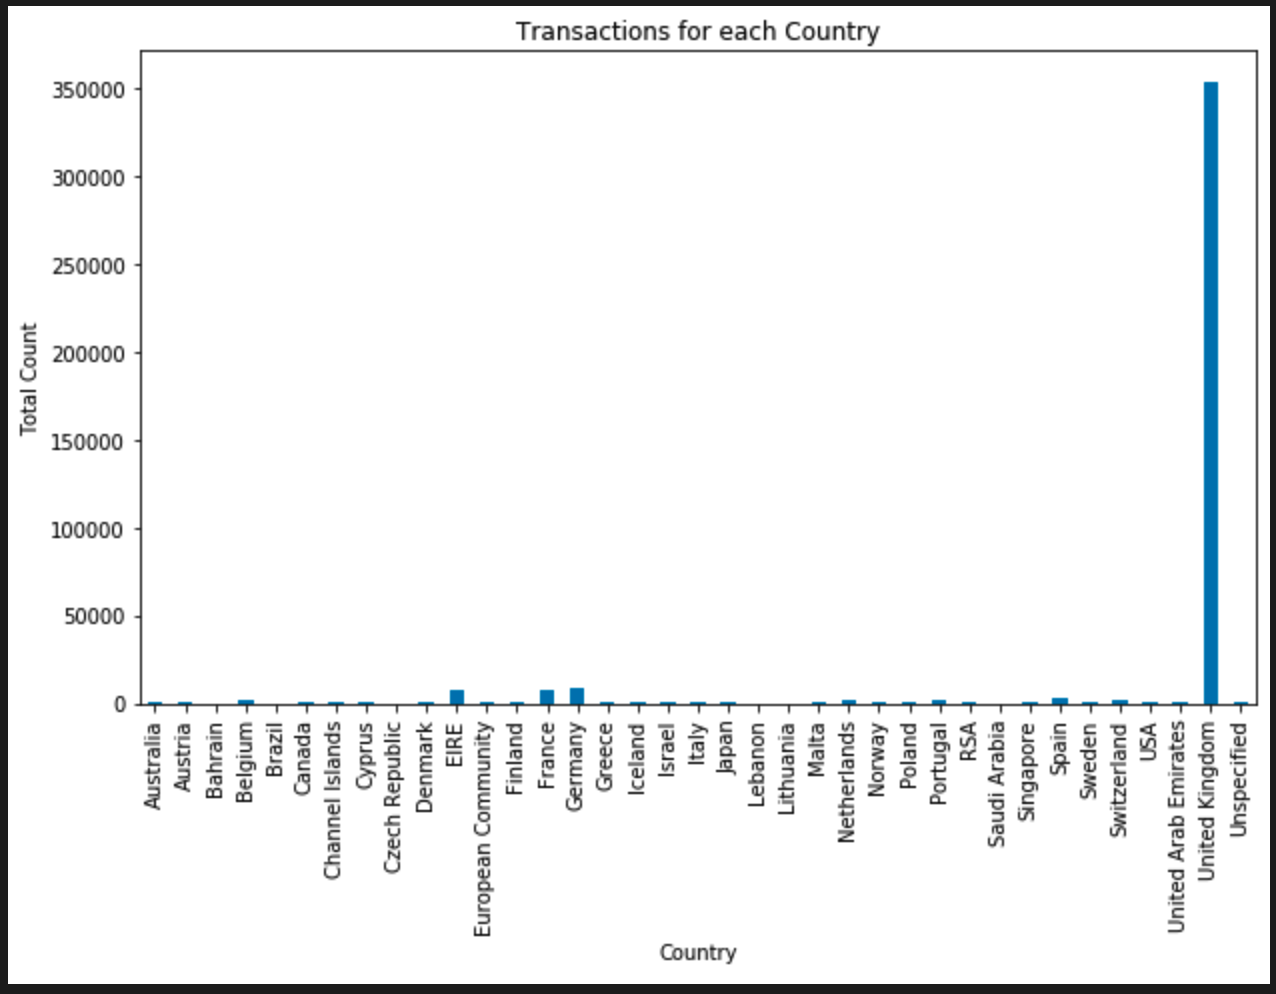
\includegraphics[scale=0.5]{totalcount}
	
	\section{\\Lift Table of Items Whole Dataset}
	\label{appendix:wholelift}
	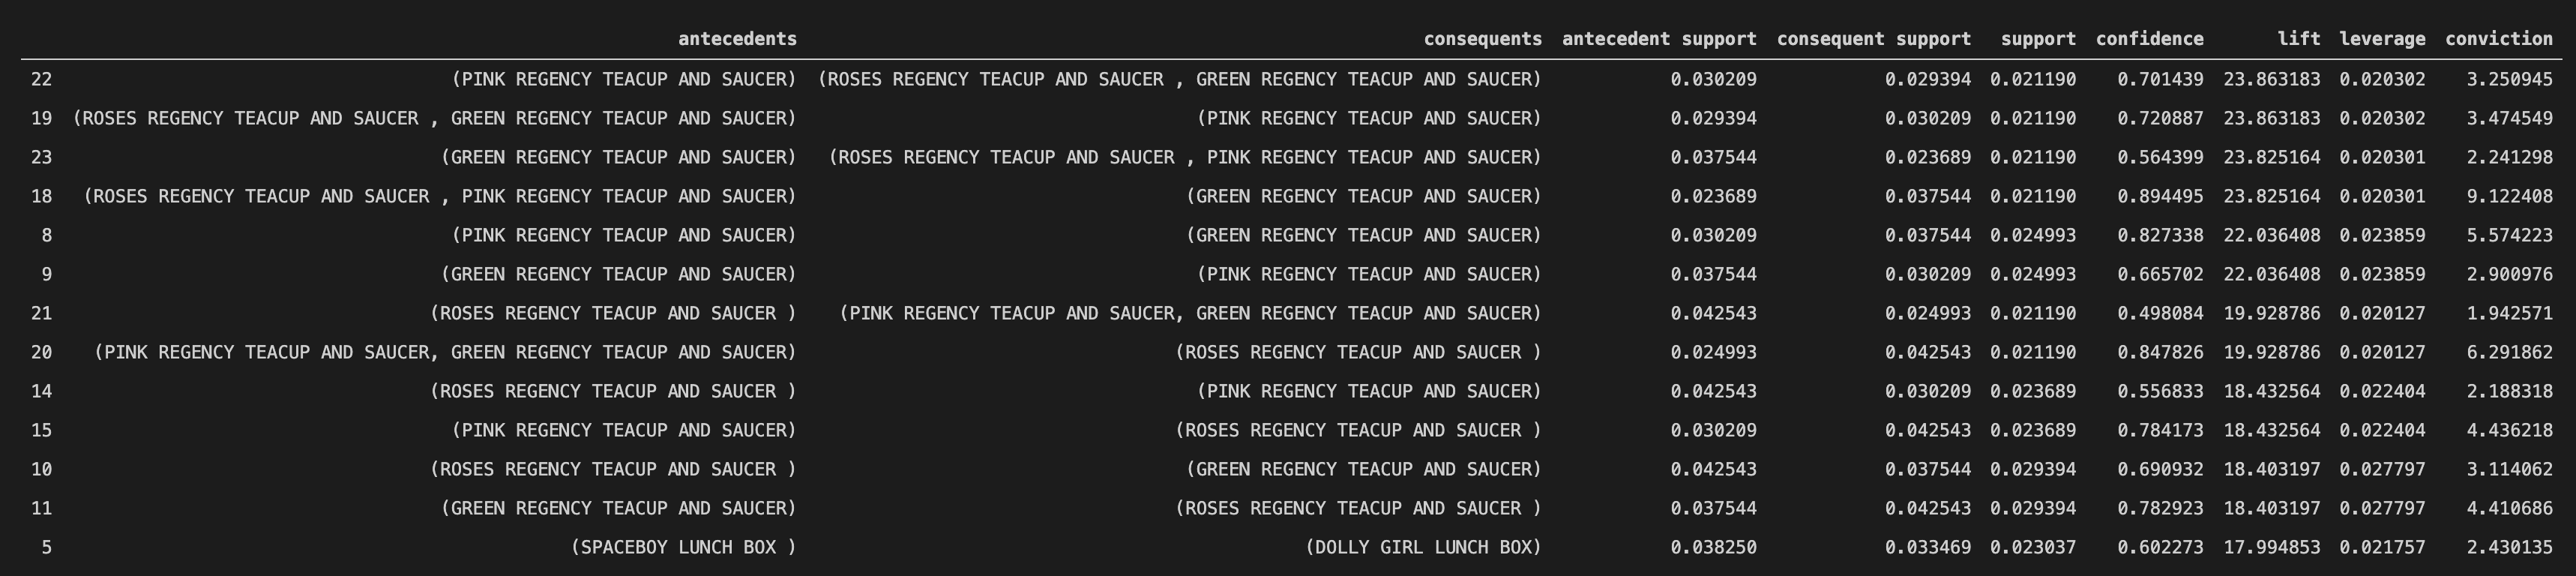
\includegraphics[scale=0.2]{wholelift}
	
	\section{Confidence Table of Items Whole Dataset}
	\label{appendix:wholeconf}
	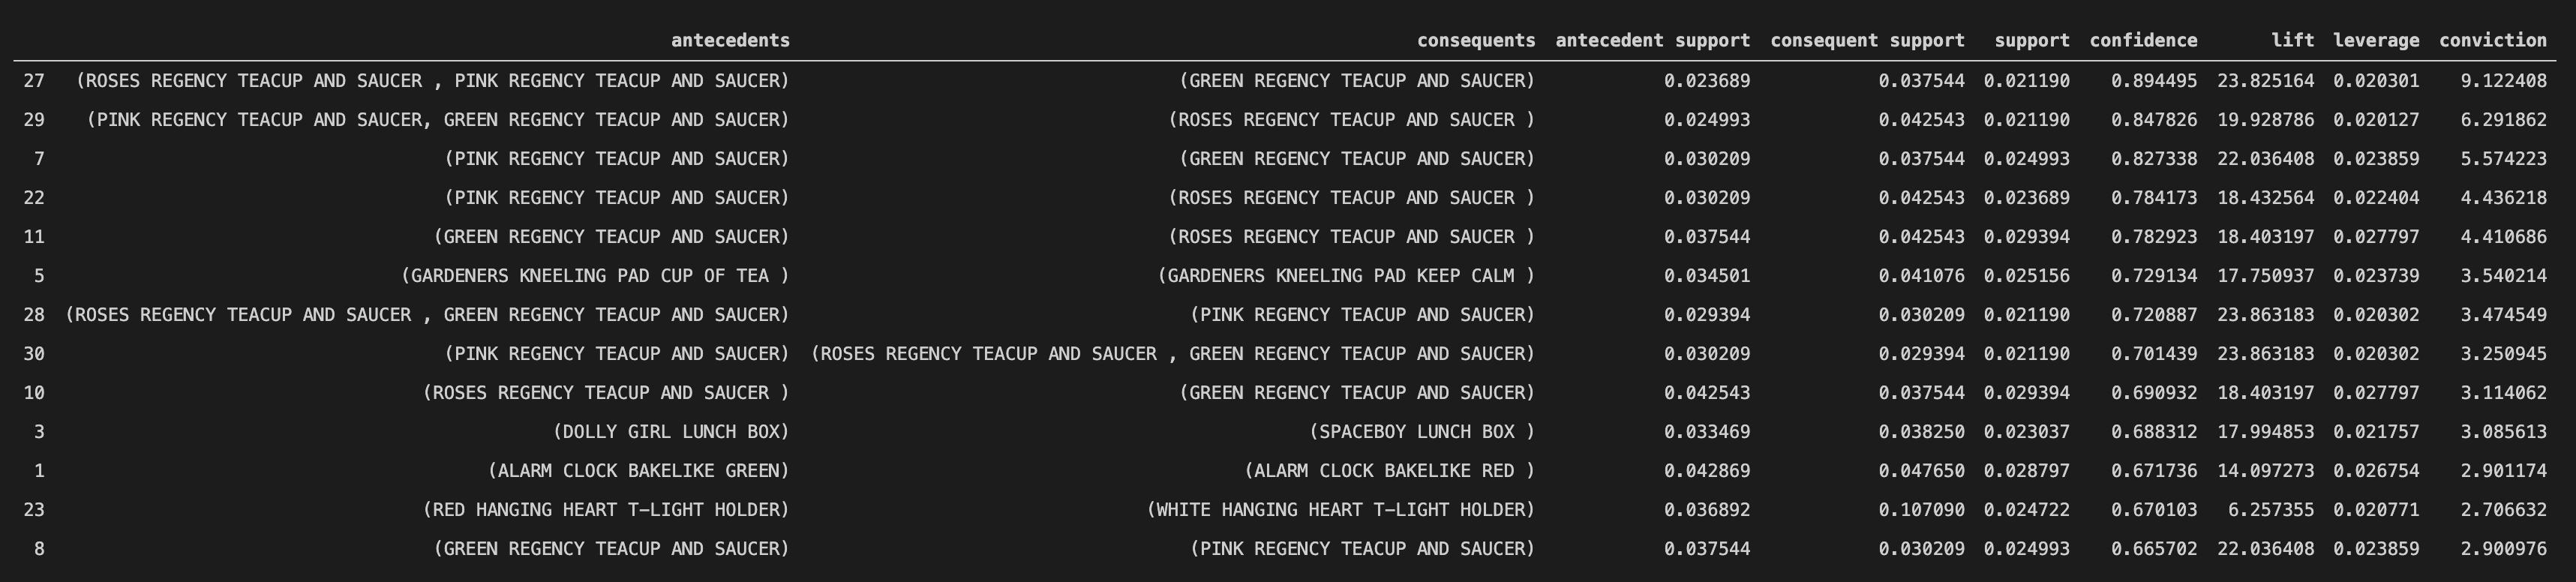
\includegraphics[scale=0.2]{wholeconf}
	
\end{appendices}

\newpage

%Sets the bibliography style to UNSRT and imports the 
%bibliography file "samples.bib".
\bibliographystyle{acm}
\bibliography{samples}

\end{document}